\documentclass[12pt]{article}
%\usepackage{graphicx}
\usepackage{indentfirst}
\usepackage[export]{adjustbox}
\usepackage{graphicx}
\usepackage{float}
\usepackage{hyperref}

%opening
\title{Audio effects library\\Requirements specification}
\author{Kacper Harezga, Ewa Kobiela, Jan Laskowski\\Krzysztof Sobczyk, Grzegorz Machura}
\date{10.04.2021}
\begin{document}
	
	\maketitle
	\tableofcontents
	\newpage
	
\section{Project constraints}

\subsection{Project requirements document}	
	
	\begin{figure}[H]
		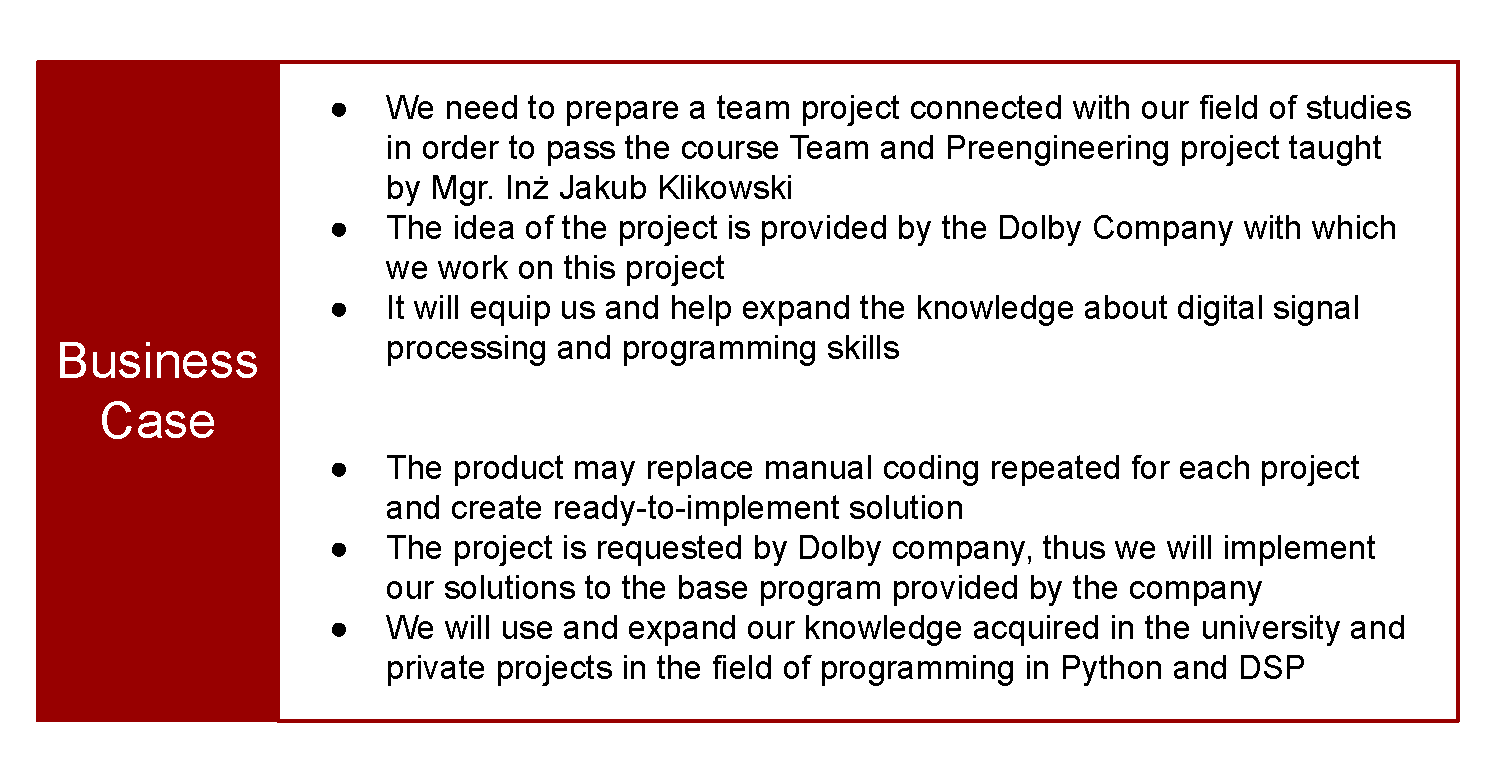
\includegraphics[width=1\textwidth, center]{Business Case Expanded}
	\end{figure}
	
	\begin{figure}[H]
		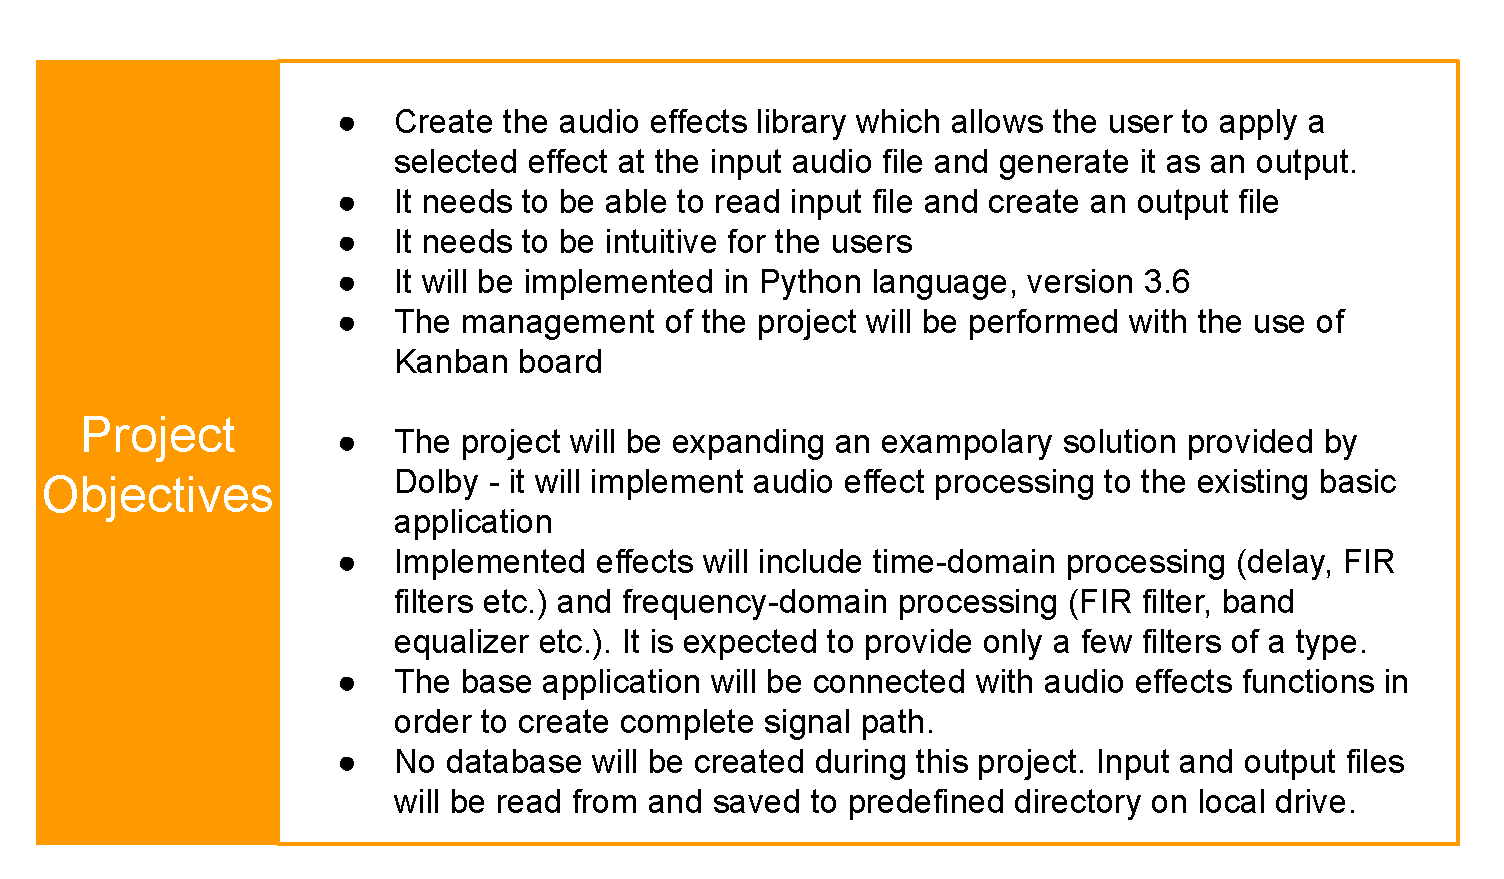
\includegraphics[width=1\textwidth, center]{Project Objectives Expanded}
	\end{figure}
	
	\begin{figure}[H]
		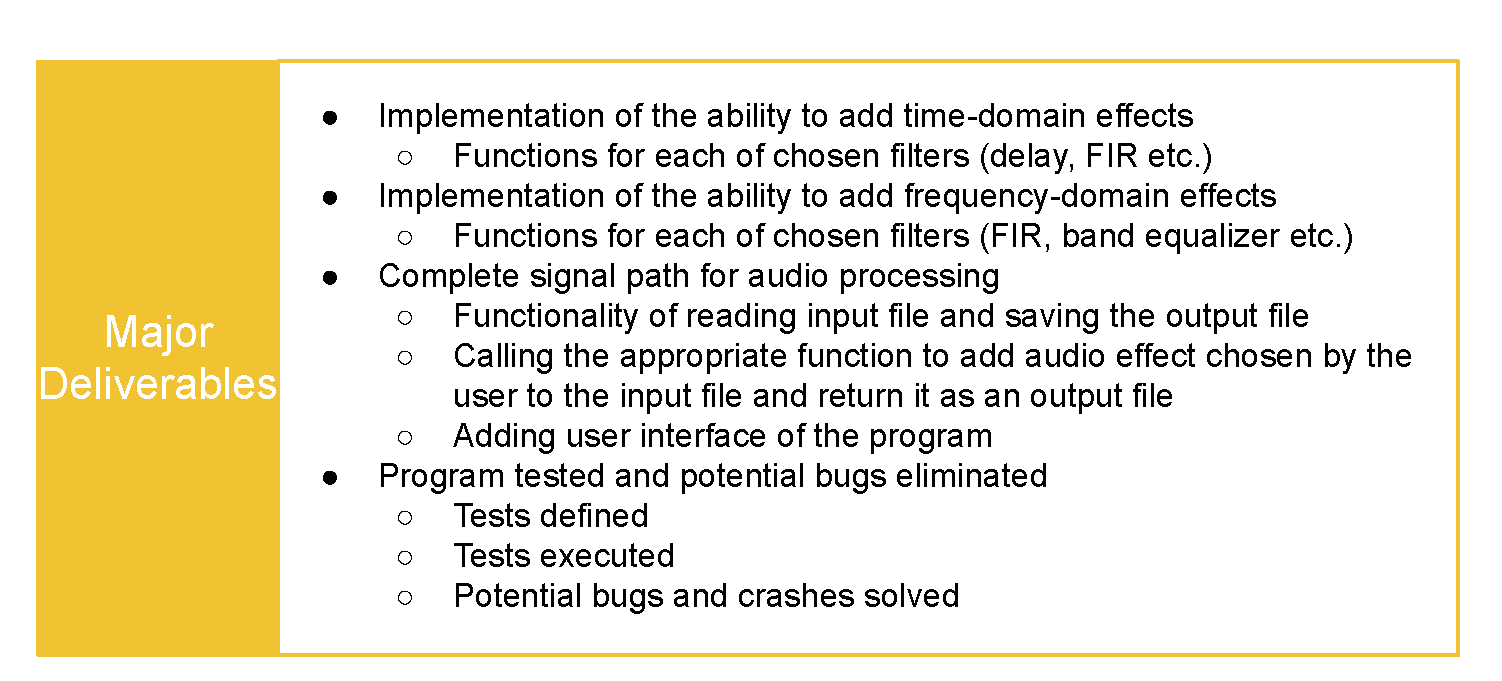
\includegraphics[width=1\textwidth, center]{Major Deliverables}
	\end{figure}
	
	\begin{figure}[H]
		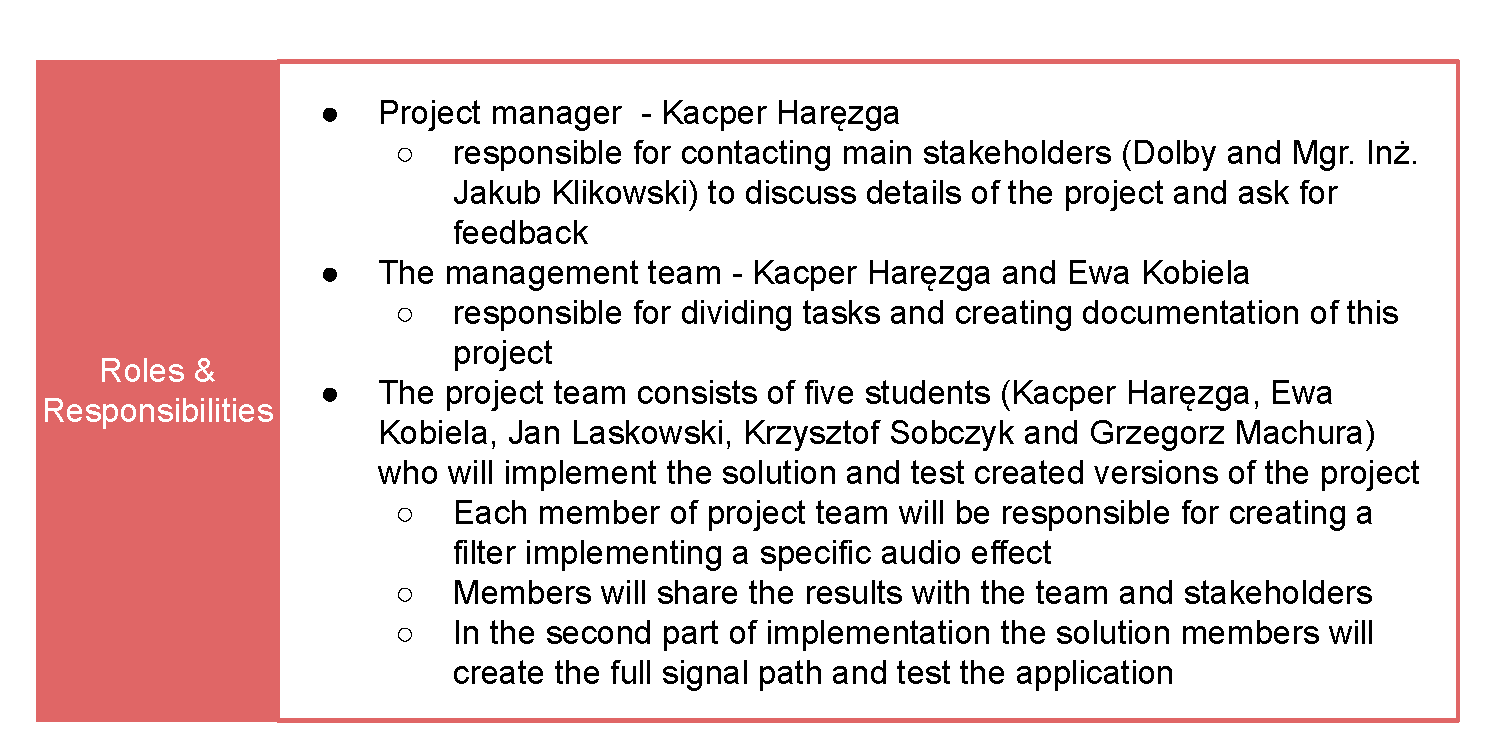
\includegraphics[width=1\textwidth, center]{Roles & Responsibilities (1)}
	\end{figure}
	
	\begin{figure}[H]
		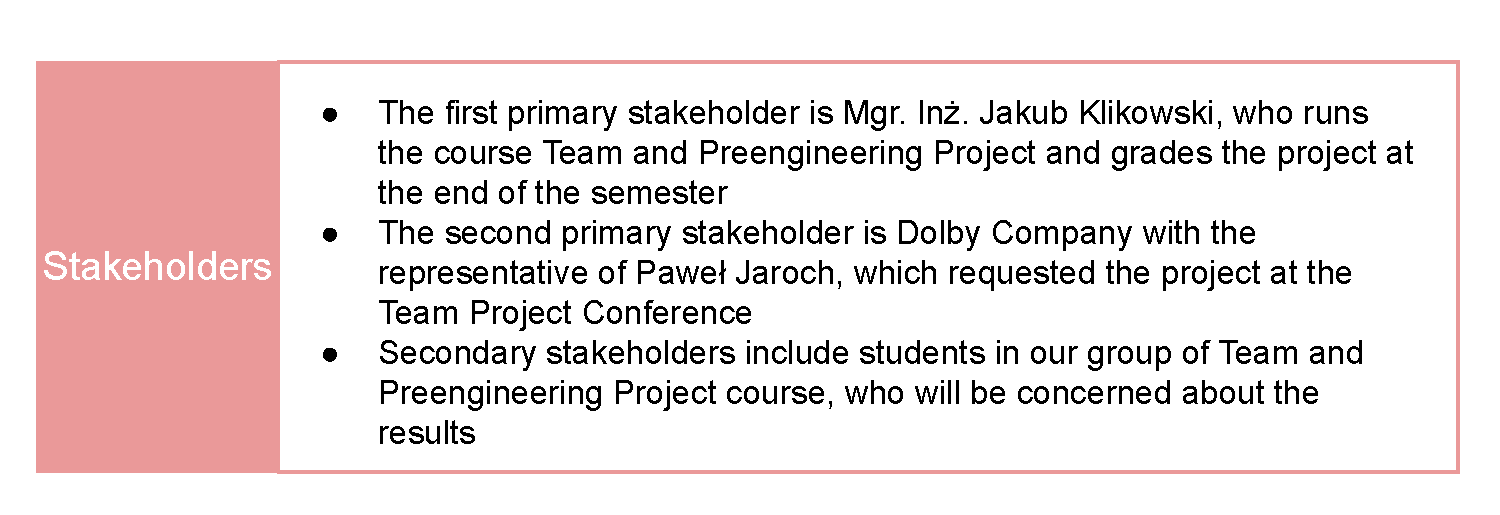
\includegraphics[width=1\textwidth, center]{Stakeholders}
	\end{figure}
	
	\begin{figure}[H]
		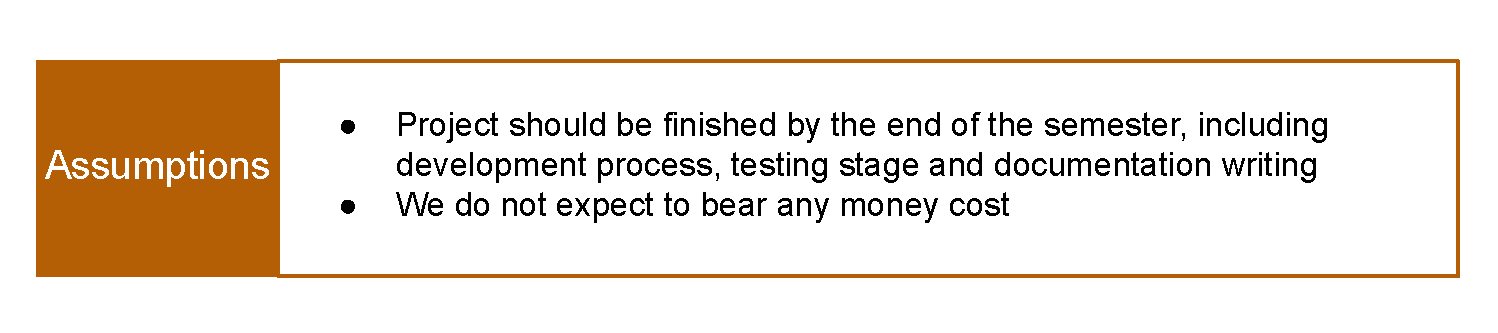
\includegraphics[width=1\textwidth, center]{Assumptions}
	\end{figure}

\subsection{Mandated constraints}

It is anticipated to create a single version of product which will contain all functionalities described in this document. Additionally, the development process will be divided in two increments, after which Dolby Laboratories Inc. will have opportunity to provide feedback and point possible improvement of the project. First increment will end once time domain filters will be implemented. The scope of second increment will expand the functionality of the application with frequency domain processing filters and simple interface to test or present possibilities of the system.

Programming language used in the project was chosen by the stakeholder - which is Dolby Laboratories Inc. - to be Python. Due to the need to use specific libraries for this language we agreed on version 3.6 of Python. Tools used in development process was chosen to consist of PyCharm by JetBrains as IDE and for GIT for version control.

The product shall use a simple pipeline, which will process an input sound file into an output sound file, adding a chosen effect in the process. The system will not work on real-time mode, thus the input file must be prepared by the client ahead. The library will be used by the client in post-production of sound, music or movies, thus additional real-time frequency will not be required. All files generated as output signals must be audible, saved in the sound file type. We do not assume any reverting functionality, i. e. removing effect from the output signal. It is important to allow user to choose the appropriate effect(s) for their application, thus the choosing dialogue must be clear and user-friendly.

The designed system might be a part of a bigger system. To achieve that effect, the external application must support file reading or/writing. The input files must be placed in a predefined directory required by Audio Effect Library's pipeline and the output files will be saved to another predefined directory, thus the external application must be able to read and/or write files with sound types of extensions to/from this directory.

The Audio Effect Library system could be used on personal computers in the form of scripts using and IDE. In this form the application would be stand-alone, however it would require from the potential user a set of IT skills and installing additional software such as IDE to run the application. The second way to implement the system is to use it on a microcontroller as a part of a bigger sound system.

Scheduled constrains of this project is set to the end of a summer semester 2020-2021, i. e. 22.06.2021, which is a critical data of finishing all the work. In case of any unexpected adversities that would make it impossible to finish all planned functionalities by this date, the project would be released in the current state, as the deadline is final. Such a deadline is required by the university and the need for grading the project and finishing the course. However, the plan assumes finishing the process of development by the end of May to reserve time for testing procedures and applying feedback or performance investigation of the system.

Budget of this project do not assume any expenses that the project team would take, besides energy consumed by the devices and maintenance costs of them. We intend to use only the software with open licences, such as GIT, or provided by the university, such as PyCharm IDE.

\subsection{Work breakdown structure}

\begin{figure}[H]
		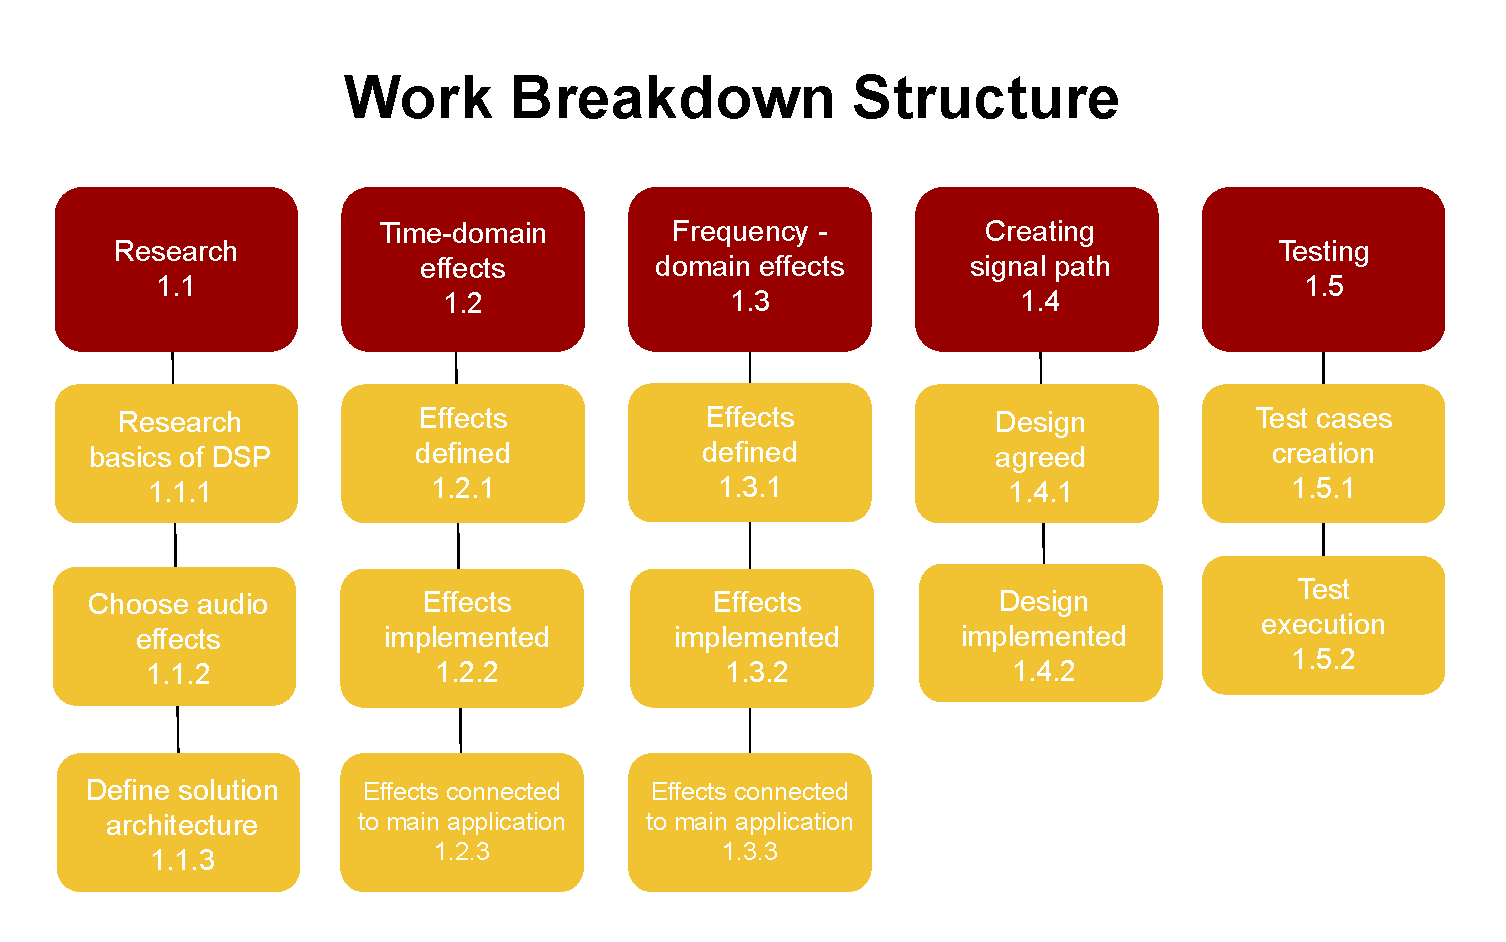
\includegraphics[width=1.2\textwidth, center]{WBS}
\end{figure}

\subsection{Naming conventions and terminology}

In order to avoid misunderstanding of scope of each work package from provided work breakdown structure, we present below the dictionary of the convention and terminology.

\begin{figure}[H]
		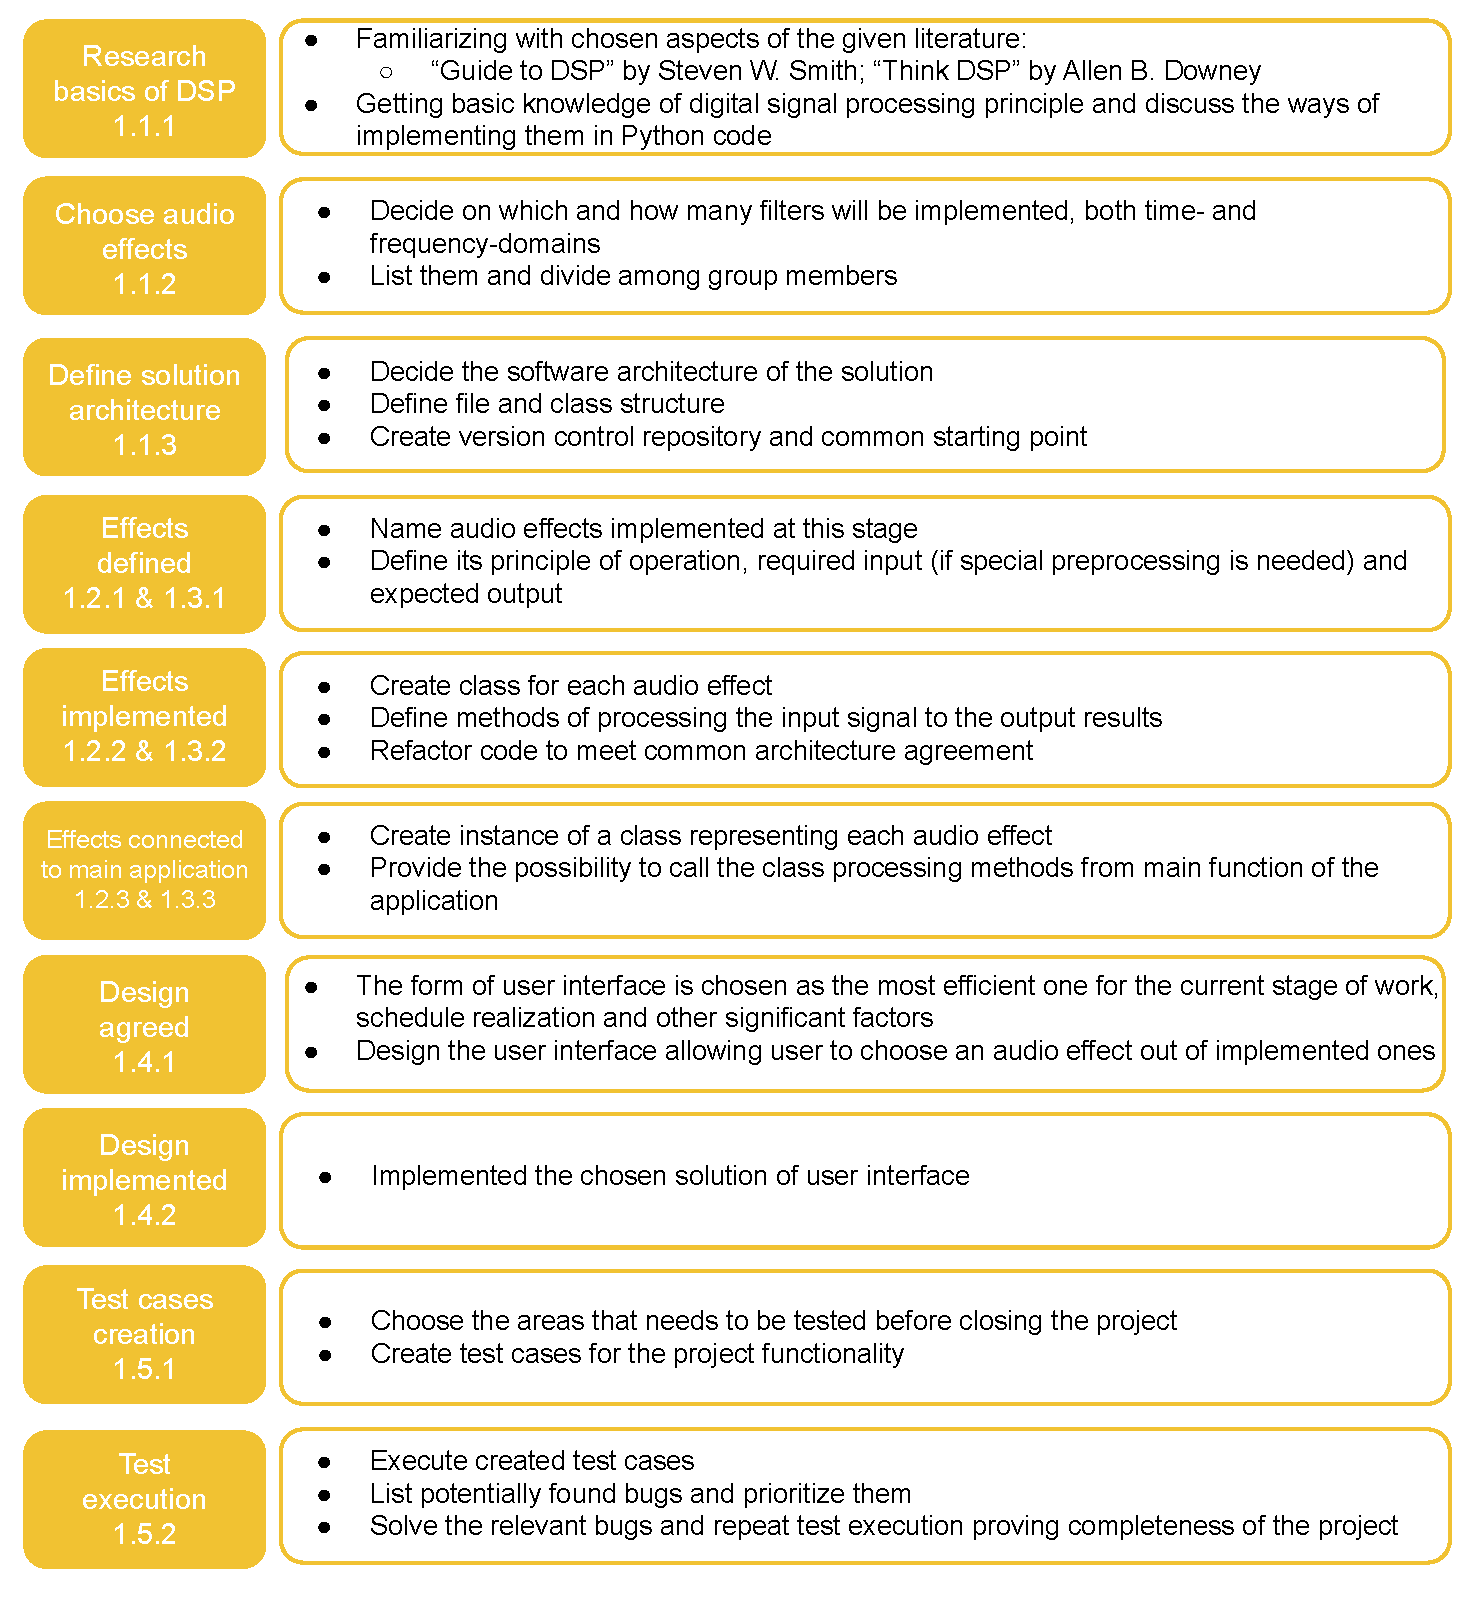
\includegraphics[width=1.2\textwidth, center]{WBS dictionary}
\end{figure}

\subsection{Relevant facts and assumptions}

An exemplary pipeline is provided by Dolby Laboratories Inc. That consists of a set of scripts processing an input signal by reducing each audio frame by a half. The team's task is to extend this simple application to allow wider range of audio processing effects. The assumption is not to write the main function from scratch, but to extend the one provided by Dolby company. We will build on basis on that and expand the project with feature files.

	Another relevant assumption is that no money cost is predicted. The software used in this project will contain free licence programs (such as Git version control system) or with licence provided by university (such as PyCharm IDE by JetBrains).
	
	Moreover, the non-exceeding deadline for finishing the project is 13.06.2021 which is the end of current university semester.

\section{Functional Requirements}

\begin{figure}[H]
		\includegraphics[width=1.2\textwidth, center]{Project scope statement}
\end{figure}

\subsection{Scope of the work}

	The workload in this project consists mainly of creating the product with constraints agreed with the stakeholders. The product should be fully functional with complete sognal path, ability to read/write files and add an audio effect chosen by the user to the main signal. The application must be fully tested and potentially relevant bugs should be eleiminated before finishing the project.
	
	Moveover, the project scope will include achieveing the ecceptance of the project by the stakeholders, both Dolby and University side. After receiving feedback for each step we will implement the comments and improvements. Moreover, after the stage of testing all potential bugs should be closed.
	
	Besides implementing the technical solutions, the docummentation of this project will be written. It will consist several stages and feedback to them will be included in the final form of project docummentation.
	
	Finally, we will collect knowledge gained in this project. All personal experiences will be collected and discussed, thus strong and weak points of technical solution, project management and any other concerned field will be known and we will sum up the benefits of this project duration.

\subsection{Business data model}

The Audio Effects Library is not be using any additional database. The input and output files are stored in project directories and can be modified directly in the file explorer. The application downloads file with a given name from the folder "input" and after processing the signal it writes a file containing new data into the folder "output", using the same filename as of the input file. This allows user to easily recognize the processed data in the directory. In case of processing the same input file for the second time, the output file is overwrite with the new type of processing. The input signal may be either stereo (for example music) or mono (for example speech) type of signal.

\subsection{Data dictionary}

Dictionary of data names used in the project is presented in the table below.

\begin{figure}[H]
		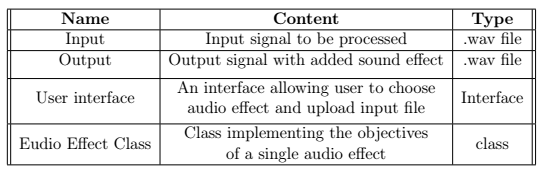
\includegraphics[width=1\textwidth, center]{Data dictionary}
\end{figure}

%\begin{table}
%	\begin{tabular}{||c| c |c||}
%		\hline
%		\textbf{Name} & \textbf{Content} & \textbf{Type} \\ 
%		\hline
%		Input & Input signal to be processed & .wav file \\ 
%		\hline
%		Output & Output signal with added sound effect & .wav file \\ [1ex] 
%		\hline
%		User interface & \makecell{An interface allowing user to choose \\ audio effect and upload input file}  & Interface \\ [2ex] 
%		\hline
%		Eudio Effect Class  & \makecell{Class implementing the objectives \\ of a single audio effect} & class \\ [1ex] 
%		\hline
%	\end{tabular}
%\end{table}

\subsection{Scope of the product}

	The product consists of a stand-alone desktop application implementing a functionality of adding chosen audio effect to the input .wav file. The application will generate an output .wav file being a result of addition of the input signal and audio effect. The set of possible effects is finite and will be displeyed to the user. The list will contain only the effect being in the scope of this project.
	
	The deliverable consist of Python scripts bein a prototype of the application and specific place noted for transfering input files and receiving output files. There are no database implemented. The packet handled to stakeholders will contain also docummentation of the project, description of the prototype including short manual for instalation and usage.

\subsection{Functional requirements}

	The main functionality is defined as converting input files into outputs with added chosen audio effect. The success criteria of this functionality is that the full signal path is created and user is allowed to choose an effect from the list of implemented ones. User will know where to put the input file and where to find the output file. Both of them should be in .wav format.

\section{Non-functional Requirements}

\subsection{Look and feel requirements}

	The product will not implement any physical features, thus feel requirements does not apply.
	
	Feel requirements are defined as a simple user interface application. User should get the information where to place the input file, which format is supported, where to find the output file. The user should be able to recognize the place to choose an effect to be implemented and be able to use it. The apperance requirements such as colours or brandings are not defined and may be choosen freely.

\subsection{Usability and humanity requirements}

	The user should be able to use this product quiclky when installed on the computer. No preparation should be required for the user, if they come with a .wav file with signal to be processed. The casual user should only remember to have the correct format of the file, as the product will not support any other file types.
	
	The application should generate a minimum amount of errors and the output files should be possible to be recognized which effect was used when creating the specific file. The product can help the user to avoid making mistakes when implementing the audio effect independently. The effects avaliable in the product will be strictly defined and missunderstandings of the process of digital signal processing by the user will be decreased. The product shall be used by people with basic understand of English and computer skills, with no advanced knowledge about digital signal processing on electroacoustics.

\subsection{Performance requirements}

	The speed of operation of the product shall be less than few minutes. The response of the system to the user decision to process the input signal shall be immidiate. However, the time of processing the signal, aspecially large files is allowed to take up to seconds or minutes. We set a treshold for the system to generate the output file to maximum of five minutes for lagre files for 90 percent of the interrogations. The product shall be avaliable to operate at any time, after the previous processing has ended.

\subsection{Operational and environmental requirements}

	The product shall work on the last releases of Windows operating systems. We do not support any other systems than Windows at this point. We will test the functionality of the product on Windows 10.
	
	Our product shall be distributed as a ZIP file. The installation and operating intruction shall be delivered with the product files to allow user safely and properly installation and usage of the application.
	
	We do not predict to maintain the product after release and acceptance by the Dolby company and University party. Only one release is planned.

\subsection{Maintainability and support requirements}

	The maintenance shall be done only by the application creators. We do not support any changes done by the user, which include adding, deleting or changing any source files. The user is allowed to save files in a given directory at any time. The product is intended to be used by private users in the Windows operating systems.

\subsection{Security requirements}

	Only creators of the application shall access and change source files. The product shall prevent incorrect file formats to being processed in order to avoid crashes of the application. The product is not intended to store or process any personal or sensitive data, thus no data security mechanisms will e provided. The concern of processing copyright files such as songs etc. is in the user's responsibility. The product creators does not take reponsibility for using the product to process copyright files.

\subsection{Cultural and legal requirements}

	The product shall not be offensive to any social group. The product shall not be used for illegal purposes and with copyright data.
	
\end{document}